%==============================================================================
%  Supplemental Material for the course report "Kitaev Honeycomb model"
%  Detailed derivations, lattice conventions, and additional figures
%  referenced from main.tex as [SM].
%
%  Compile:  pdflatex supplement ; bibtex supplement ; pdflatex x2
%==============================================================================
\documentclass[
  aps,
  prl,
  preprint,
  amsmath,
  amssymb,
  superscriptaddress,
  floatfix
]{revtex4-2}

\usepackage{graphicx}
\usepackage{float}
\usepackage{tikz}
\usetikzlibrary{calc}
\usetikzlibrary{arrows.meta}
\usepackage{bm}
\usepackage{braket}
\usepackage{physics}
\usepackage{xcolor}
\usepackage[colorlinks=true,allcolors=blue]{hyperref}
\usepackage[capitalise]{cleveref}

\graphicspath{{figures/}{../Note/Plots/}{../Plots/}}

% --- macros (subset of main.tex) ----------------------------------------------
\newcommand{\Z}{\mathbb{Z}}
\newcommand{\ii}{\mathrm{i}}
\newcommand{\ee}{\mathrm{e}}
\newcommand{\pp}{\partial}
\newcommand{\oga}{\hat \gamma}
\newcommand{\obx}{\hat b^x}
\newcommand{\oby}{\hat b^y}
\newcommand{\obz}{\hat b^z}
\renewcommand{\oc}{\hat{c}}
\newcommand{\oK}{\hat{K}}
\newcommand{\oA}{\hat{A}}
\newcommand{\oH}{\hat{H}}
\newcommand{\oT}{\hat{T}}
\newcommand{\oI}{\hat{\mathbb{I}}}
\newcommand{\C}{\mathcal{C}}
\newcommand{\sgn}{\operatorname{sgn}}
\renewcommand{\abs}[1]{\left| #1 \right|}
\renewcommand{\comm}[2]{\left[ #1 , #2 \right]}
\newcommand{\anticomm}[2]{\left\{ #1 , #2 \right\}}
\newcommand{\mean}[1]{\left\langle #1 \right\rangle}
\newcommand{\numberthis}{\refstepcounter{equation}\tag{\theequation}}

% --- S-numbering ---------------------------------------------------------------
\renewcommand{\thesection}{S\Roman{section}}
\renewcommand{\thefigure}{S\arabic{figure}}
\renewcommand{\theequation}{S\arabic{equation}}

\begin{document}

\title{Supplemental Material:\\ Kitaev Honeycomb Model}
\author{Zhenming Shi}
\affiliation{Leipzig University}
\date{\today}
\maketitle

% Number sections so that \cref/\ref to \label{sm:...} resolve (PRL suppresses
% section numbers by default, which leaves section cross-references blank).
\setcounter{secnumdepth}{3}

This Supplemental Material is to present the details to prove personal understanding.
\section{Derivations about the commutator and eigenvalues}

The plaquette operator has the equivalent expression:
\begin{align*}
    \hat W_p &= \oK_{12} \oK_{23} \oK_{34} \oK_{45} \oK_{56}\oK_{61} \\
    &= \sigma_1^z \sigma_2^z \sigma_2^x \sigma_3^x \sigma_3^y \sigma_4^y \sigma_4^z \sigma_5^z \sigma_5^x \sigma_6^x \sigma_6^y \sigma_1^y \\
    &= (\sigma_1^z \sigma_1^y) \sigma_2^z \sigma_2^x \sigma_3^x \sigma_3^y \sigma_4^y \sigma_4^z \sigma_5^z \sigma_5^x \sigma_6^x \sigma_6^y \\
    &= (\ii \epsilon_{zyx} \sigma_1^x)(\ii \epsilon_{zxy} \sigma_2^y)(\ii \epsilon_{xyz} \sigma_3^z)(\ii \epsilon_{yzx} \sigma_4^x)(\ii \epsilon_{zxy} \sigma_5^y)(\ii \epsilon_{xyz} \sigma_6^z)\\
    &= \ii^6\,\epsilon_{zyx}\,\epsilon_{zxy}\,\epsilon_{xyz}\,\epsilon_{yzx}\,\epsilon_{zxy}\,\epsilon_{xyz}\;
       \sigma_1^x\sigma_2^y\sigma_3^z\sigma_4^x\sigma_5^y\sigma_6^z \\
    &= (-1)(-1)(+1)(+1)(+1)(+1)(+1)\;\sigma_1^x\sigma_2^y\sigma_3^z\sigma_4^x\sigma_5^y\sigma_6^z \\
    &= \sigma_1^x \sigma_2^y \sigma_3^z \sigma_4^x \sigma_5^y \sigma_6^z \numberthis
\end{align*}
The square of the plaquette operator is 
\begin{align*}
  \hat{W}_p^2 = \prod_{j=1}^{6} (\sigma_{j}^{\alpha_j})^2 = \oI
\end{align*}
thus the eigenvalues of $\hat{W}_p$ are $\pm 1$. For a bond on the hexagon,
e.g.\ the $z$-bond $\oK_{12}$, the bond label differs from the $\hat W_p$
Pauli matrix at both shared sites:
\begin{align*}
  \oK_{12}\, \hat W_p
  = (\sigma_1^z \sigma_2^z)(\sigma_1^x \sigma_2^y \sigma_3^z \sigma_4^x \sigma_5^y \sigma_6^z)
  = (-1)^2\, (\sigma_1^x \sigma_2^y \sigma_3^z \sigma_4^x \sigma_5^y \sigma_6^z)(\sigma_1^z \sigma_2^z)
  = \hat W_p\, \oK_{12}.
\end{align*}
For an outward bond, e.g.\ the $x$-bond $\oK_{11'}$ with $1' \notin p$, the
bond label matches the Pauli matrix at the single shared site:
\begin{align*}
  \oK_{11'}\, \hat W_p
  = (\sigma_1^x \sigma_{1'}^x)(\sigma_1^x \sigma_2^y \sigma_3^z \sigma_4^x \sigma_5^y \sigma_6^z)
  = (+1)\, (\sigma_1^x \sigma_2^y \sigma_3^z \sigma_4^x \sigma_5^y \sigma_6^z)(\sigma_1^x \sigma_{1'}^x)
  = \hat W_p\, \oK_{11'}.
\end{align*}
A bond which does not touch $p$ commutes trivially. Hence
\begin{align*}
  \comm{\hat{K}_{jk}}{\hat{W}_p}= 0 \qquad \implies \qquad \comm{\hat H}{\hat{W}_p} =0
\end{align*}
So the Hilbert space splits into flux sectors labelled by the eigenvalues $\{w_p\}$. By four Majorana representation, the Hamiltonian is replaced by $\tilde{H}\{\tilde{\sigma}_{j}\}$ and the bond operator becomes 
\begin{align*}
  \tilde K_{jk} = (\ii \hat b_j^\alpha \oga_j)(\ii \hat b_k^\alpha \oga_k) 
    = -\hat b_j^\alpha \oga_j \hat b_k^\alpha \oga_k 
    = \hat b_j^\alpha \hat b_k^\alpha \oga_j \oga_k 
    = -\ii (\ii \hat b_j^\alpha \hat b_k^\alpha) \oga_j \oga_k
\end{align*}
thus the Hermitian Majorana bond operator is defined by:
\begin{align*}
  \hat{u}_{jk} = \ii \hat{b}^ \alpha_j \hat{b}^ \alpha_k \qquad \hat u_{jk} ^ \dag = (\ii \hat b^\alpha_j \hat b^ \alpha_k)^ \dag = - \ii \hat b^\alpha_k \hat b^ \alpha_j = \ii \hat b^\alpha_j \hat b^ \alpha_k = \hat u_{jk}.
\end{align*}
The constraint operator $\hat D_j = \obx_j \oby_j \obz_j \oga_j$ commutes
with the bond operator. A Majorana at site $j$ commutes with its own copy
inside $\hat D_j$ and anticommutes with the other three factors. A
Majorana at $k \neq j$ anticommutes with all four:
\begin{align*}
  \hat b^\alpha_j \hat D_j &= (-1)^3\, \hat D_j\, \hat b^\alpha_j,
  &
  \oga_j \hat D_j &= (-1)^3\, \hat D_j\, \oga_j,
  \\
  \hat b^\alpha_k \hat D_j &= (-1)^4\, \hat D_j\, \hat b^\alpha_k,
  &
  \oga_k \hat D_j &= (-1)^4\, \hat D_j\, \oga_k.
\end{align*}
Hence
\begin{align*}
  \hat D_j\, \tilde K_{jk}
  &= \hat D_j\, \hat b^\alpha_j\, \hat b^\alpha_k\, \oga_j\, \oga_k \\
  &= -\hat b^\alpha_j\, \hat D_j\, \hat b^\alpha_k\, \oga_j\, \oga_k \\
  &= -\hat b^\alpha_j\, \hat b^\alpha_k\, \hat D_j\, \oga_j\, \oga_k \\
  &= +\hat b^\alpha_j\, \hat b^\alpha_k\, \oga_j\, \hat D_j\, \oga_k \\
  &= \hat b^\alpha_j\, \hat b^\alpha_k\, \oga_j\, \oga_k\, \hat D_j
   = \tilde K_{jk}\, \hat D_j,
\end{align*}
and a bond not containing $j$ commutes with $\hat D_j$ trivially, so
\begin{align*}
  \comm{\hat{D}_j}{\tilde{K}_{jk}} = 0 \qquad \implies \qquad
  \comm{\hat D_j}{\tilde H} = 0, \numberthis
\end{align*}
i.e.\ $\tilde H$ preserves the physical subspace $\hat D_j \ket{\xi} = \ket{\xi}$.
%==============================================================================
\section{Lattice conventions}
\label{sm:conventions}

The system is translation invariant under any Bravais vector $\bm R = n_1
\bm n_1 + n_2 \bm n_2$ with $n_1,n_2 \in \mathbb{Z}$. We place the odd
($A$) sublattice at the cell origin $\bm R$ and the even ($B$) sublattice
at $\bm R+\bm\delta_z$. The nearest-neighbour bond vectors
$\bm\delta_\alpha$ point from $A$ to $B$, and the primitive vectors are
$\bm n_1=\bm\delta_z-\bm\delta_y$, $\bm n_2=\bm\delta_z-\bm\delta_x$
(\cref{fig:sm_conventions}). Note $\bm\delta_x+\bm\delta_y+\bm\delta_z=0$.

\begin{figure}[H]
  \centering
  \begin{minipage}[c]{0.34\textwidth}
  \centering
  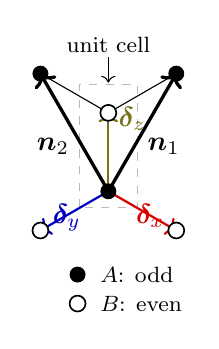
\begin{tikzpicture}[scale=1.15, line width=0.6pt]
    \colorlet{cx}{red!85!black}\colorlet{cy}{blue!75!black}\colorlet{cz}{olive!80!black}
    \coordinate (B0) at (0, 0);
    \coordinate (A0) at (0, 0.866);
    \coordinate (Aleft)  at (-0.75, 1.299);
    \coordinate (Aright) at (0.75, 1.299);
    \coordinate (Bleft)  at (-0.75, -0.433);
    \coordinate (Bright) at (0.75, -0.433);
    \draw[thin] (A0) -- (Aleft);
    \draw[thin] (A0) -- (Aright);
    \draw[thin, gray!55, dashed] (-0.32,-0.18) rectangle (0.32,1.18);
    \draw[->, thick, cz] (B0) -- (A0)     node[pos=0.92, right=0pt]   {$\bm\delta_z$};
    \draw[->, thick, cx] (B0) -- (Bright) node[midway, below right=-6pt] {$\bm\delta_x$};
    \draw[->, thick, cy] (B0) -- (Bleft)  node[midway, below left=-6pt]  {$\bm\delta_y$};
    \draw[->, very thick] (B0) -- (Aright) node[midway, below right=-2pt] {$\bm{n}_1$};
    \draw[->, very thick] (B0) -- (Aleft)  node[midway, below left=-2pt]  {$\bm{n}_2$};
    \fill (B0) circle (2.5pt);
    \fill[white] (A0) circle (2.5pt); \draw (A0) circle (2.5pt);
    \fill[white] (Bleft) circle (2.5pt); \draw (Bleft) circle (2.5pt);
    \fill[white] (Bright) circle (2.5pt); \draw (Bright) circle (2.5pt);
    \fill (Aleft) circle (2.5pt);
    \fill (Aright) circle (2.5pt);
    \node[font=\footnotesize] at (0, 1.62) {unit cell};
    \draw[->, thin] (0, 1.48) -- (0, 1.2);
    \fill (-0.34,-0.92) circle (2.5pt);
    \node[anchor=west, font=\footnotesize] at (-0.20,-0.92) {$A$: odd};
    \fill[white] (-0.34,-1.24) circle (2.5pt); \draw (-0.34,-1.24) circle (2.5pt);
    \node[anchor=west, font=\footnotesize] at (-0.20,-1.24) {$B$: even};
  \end{tikzpicture}
  \end{minipage}\hspace{2em}
  \begin{minipage}[c]{0.34\textwidth}
  \[
  \begin{aligned}
    \bm\delta_x &= \big(\tfrac{\sqrt3}{2},\, -\tfrac12\big),\\[2pt]
    \bm\delta_y &= \big(-\tfrac{\sqrt3}{2},\, -\tfrac12\big),\\[2pt]
    \bm\delta_z &= (0,\, 1),\\[5pt]
    \bm n_1 &= \big(\tfrac{\sqrt3}{2},\, \tfrac32\big),\\[2pt]
    \bm n_2 &= \big(-\tfrac{\sqrt3}{2},\, \tfrac32\big).
  \end{aligned}
  \]
  \end{minipage}
  \caption{Bond vectors $\bm\delta_\alpha$ ($A\to B$, coloured by bond
    type) and primitive Bravais vectors $\bm n_{1,2}$ of the honeycomb
    lattice, with the two-site unit cell (dashed).}
  \label{fig:sm_conventions}
\end{figure}

%==============================================================================
\section{Fourier transform, Bloch Hamiltonian, and the Dirac cones}
\label{sm:fourier}

The real-space Hamiltonian in the $u_{jk}=1$ gauge is
\begin{align}
  \tilde{H}_u = \ii \sum_{\bm R,\alpha} J_\alpha\, \oga_{\bm R}^A\, \oga_{\bm R+\bm\delta_\alpha}^B .
  \label{eq:sm_realspace}
\end{align}
The prefactor $\ii$ comes from the quadratic form
$\tfrac{\ii}{4}\sum_{j,k}A_{jk}\oga_j\oga_k$ with $A_{jk}=2J_\alpha u_{jk}$,
$u_{jk}=+1$, after removing the double counting of each bond. Here I use the
\emph{periodic gauge} for the Fourier transform, so each Majorana
carries the phase of its physical position:
\begin{align}
  \oga_{\bm R}^A = \frac{1}{\sqrt{N}}\sum_{\bm q} \ee^{\ii \bm q\cdot \bm R}\, \tilde\gamma_{\bm q}^A,
  \qquad
  \oga_{\bm R+\bm\delta_\alpha}^B = \frac{1}{\sqrt{N}}\sum_{\bm q} \ee^{\ii \bm q\cdot (\bm R + \bm\delta_\alpha)}\, \tilde\gamma_{\bm q}^B,
  \qquad (\tilde\gamma_{\bm q}^{A,B})^\dag=\tilde\gamma_{-\bm q}^{A,B}.
  \label{eq:sm_FT}
\end{align}
Substitute and sum over $\bm R$,
\begin{align}
  \tilde H_u &= \frac{\ii}{N}\sum_{\bm R,\alpha} J_\alpha \sum_{\bm q,\bm q'} \ee^{\ii \bm q \cdot \bm R} \ee^{\ii \bm q' \cdot (\bm R + \bm\delta_\alpha)}\, \tilde{\gamma}_{\bm q}^A \tilde{\gamma}_{\bm q'}^B \notag\\
  &= \frac{\ii}{N} \sum_{\alpha} J_\alpha \sum_{\bm q,\bm q'} \ee^{\ii \bm q' \cdot \bm\delta_\alpha}\, \tilde{\gamma}_{\bm q}^A \tilde{\gamma}_{\bm q'}^B \underbrace{\sum_{\bm R} \ee^{\ii (\bm q + \bm q') \cdot\bm R }}_{N\,\delta_{\bm q+\bm q',\,0}}
  = \ii \sum_\alpha J_{\alpha} \sum_{\bm q} \ee^{-\ii \bm q \cdot \bm\delta_\alpha}\, \tilde{\gamma}_{\bm q}^A \tilde{\gamma}_{-\bm q}^B .
\end{align}
We split the $\bm q$-sum over $\bm q$ and $-\bm q$ and use
$\tilde\gamma_{-\bm q}^A \tilde\gamma_{\bm q}^B =
-\tilde\gamma_{\bm q}^B \tilde\gamma_{-\bm q}^A$. This gives a
Hermitian form
\begin{align}
  \tilde H_u &= \frac{\ii}{2}\sum_\alpha J_\alpha \sum_{\bm q}\left( \ee^{-\ii \bm q\cdot\bm\delta_\alpha}\, \tilde\gamma_{\bm q}^A \tilde\gamma_{-\bm q}^B + \ee^{\ii \bm q\cdot\bm\delta_\alpha}\, \tilde\gamma_{-\bm q}^A \tilde\gamma_{\bm q}^B \right) \notag\\
  &= \frac{\ii}{2}\sum_\alpha J_\alpha \sum_{\bm q}\left( \ee^{-\ii \bm q\cdot\bm\delta_\alpha}\, \tilde\gamma_{\bm q}^A \tilde\gamma_{-\bm q}^B - \ee^{\ii \bm q\cdot\bm\delta_\alpha}\, \tilde\gamma_{\bm q}^B \tilde\gamma_{-\bm q}^A \right).
\end{align}
Choosing the sublattice spinor
\begin{align}
  \chi_{\bm{q}} = \begin{pmatrix}
        \tilde\gamma_{\bm{q}}^{A} \\[4pt]
        \tilde\gamma_{\bm{q}}^{B}
    \end{pmatrix},
    \quad \chi_{\bm q}^{\dag} = \begin{pmatrix} \tilde\gamma_{-\bm q}^{A} & \tilde\gamma_{-\bm q}^{B} \end{pmatrix},
    \label{eq:sm_spinor}
\end{align}
the Hamiltonian takes the Bloch form of the main text,
\begin{align}
  \tilde{H}_u = \frac{1}{2} \sum_{\bm q} \chi_{\bm q}^\dag h(\bm q) \chi_{\bm q}, \qquad h(\bm q) = \begin{pmatrix}
    0 & \ii f(\bm q) \\
    - \ii f(\bm q)^* & 0
  \end{pmatrix},
  \label{eq:sm_bloch}
\end{align}
with
\begin{align}
  f(\bm q) = \sum_\alpha J_\alpha \ee^{\ii \bm q\cdot\bm\delta_\alpha}
  = J_x \ee^{\ii(\sqrt{3}q_x - q_y)/2}
           + J_y \ee^{-\ii(\sqrt{3}q_x + q_y)/2}
           + J_z \ee^{\ii q_y}.
  \label{eq:sm_fq}
\end{align}
The bulk dispersion $\epsilon_\pm(\bm q)=\pm\abs{f(\bm q)}$ is explicitly
\begin{align}
  \abs{f(\bm{q})}^2 = J_x^2 + J_y^2 + J_z^2
      + 2J_xJ_y\cos\!\left(\sqrt{3}\,q_x\right)
      + 2J_xJ_z\cos\!\left(\tfrac{\sqrt{3}\,q_x - 3q_y}{2}\right)
      + 2J_yJ_z\cos\!\left(\tfrac{\sqrt{3}\,q_x + 3q_y}{2}\right).
\end{align}

Expanding $h(\bm q)=\bm d(\bm q)\cdot\bm\sigma$, the components:
\begin{align}
  d_x(\bm q) &= -\operatorname{Im} f(\bm q) = -\sum_\alpha J_\alpha \sin(\bm q\cdot\bm\delta_\alpha), \notag\\
  d_y(\bm q) &= -\operatorname{Re} f(\bm q) = -\sum_\alpha J_\alpha \cos(\bm q\cdot\bm\delta_\alpha),
  \qquad
  d_z(\bm q) = 0 .
  \label{eq:sm_dvector}
\end{align}
The vanishing of $d_z$ is the chiral symmetry $\sigma_z
h(\bm q)\sigma_z=-h(\bm q)$: $\bm d$ stays in the $xy$-plane over the
whole Brillouin zone. Equivalently $d_x+\ii d_y=-\ii f^*(\bm q)$.

At the symmetric point $J_x=J_y=J_z\equiv J$, $f=0$ gives 
\begin{align}
  \ee^{\ii\phi_x}+\ee^{\ii\phi_y}+\ee^{\ii\phi_z}=0,
  \qquad \phi_\alpha \equiv \bm q\cdot\bm\delta_\alpha :
\end{align}
three unit vectors summing to zero form an equilateral triangle, so the
phases differ by $\pm2\pi/3$. We choose
\begin{align}
  \phi_x=-\tfrac{2\pi}{3},\qquad \phi_y=0,\qquad \phi_z=\tfrac{2\pi}{3} .
\end{align}
Other assignments give the same points up to reciprocal-lattice vectors.
The component equations $\bm q\cdot\bm\delta_z=q_y=\tfrac{2\pi}{3}$ and
$\bm q\cdot\bm\delta_y=-\tfrac{\sqrt3}{2}q_x-\tfrac12 q_y=0$ give
\begin{align}
  \bm q^* \equiv \pm\bm K,
  \qquad
  \bm K = \Big(-\frac{2\pi}{3\sqrt3},\ \frac{2\pi}{3}\Big),
\end{align}
the two inequivalent corners of the Brillouin zone.

Expanding $f(\bm K+\delta\bm q)\simeq f(\bm K)+\delta\bm q\cdot\nabla
f|_{\bm K}$ with
\begin{align}
  \nabla f(\bm q) = \ii J \sum_\alpha \bm\delta_\alpha\, \ee^{\ii \bm q\cdot\bm\delta_\alpha},
\end{align}
we evaluate at $\bm K$ using the three phases above:
\begin{align}
  \nabla f|_{\bm K}
  &= \ii J\Big(\bm\delta_x\, \ee^{-\ii 2\pi/3} + \bm\delta_y + \bm\delta_z\, \ee^{\ii 2\pi/3}\Big) \notag\\
  &= \ii J \left[ \Big(\tfrac{\sqrt3}{2},-\tfrac12\Big)\Big(-\tfrac12-\ii\tfrac{\sqrt3}{2}\Big)
     + \Big(-\tfrac{\sqrt3}{2},-\tfrac12\Big)
     + (0,1)\Big(-\tfrac12+\ii\tfrac{\sqrt3}{2}\Big)\right] \notag\\
  &= \frac{3J}{4}\Big(1-\sqrt3\,\ii,\ -\sqrt3-\ii\Big).
\end{align}
Hence, with $f(\bm K)=0$,
\begin{align}
  f(\bm K+\delta\bm q)
  &\simeq \frac{3J}{4}\Big[(1-\sqrt3\,\ii)\,\delta q_x + (-\sqrt3-\ii)\,\delta q_y\Big] \notag\\
  &= \frac{3J}{2}\Big(\tfrac12-\ii\tfrac{\sqrt3}{2}\Big)(\delta q_x-\ii\,\delta q_y)
  = \frac{3J}{2}\, \ee^{-\ii\pi/3}\, (\delta q_x - \ii\,\delta q_y).
  \label{eq:sm_linearization}
\end{align}
The same expansion at $-\bm K$ gives $\delta q_x+\ii\,\delta
q_y$, since $f(-\bm q)=f(\bm q)^*$. The dispersion is an isotropic Dirac
cone
\begin{align}
  \epsilon(\bm K+\delta\bm q) \simeq \frac{3J}{2}\,\abs{\delta\bm q},
  \qquad v_F=\frac{3J}{2},
\end{align}
as in graphene (\cref{fig:sm_dirac_cone}).

\begin{figure}[H]
  \centering
  \includegraphics[width=0.85\textwidth]{HC_2_dirac_cone.pdf}
  \caption{Dirac cone at the Brillouin-zone corner $\bm K$ for $J_x=J_y=J_z$.
    Left: $\abs{f(\bm q)}$ over the first BZ, vanishing at the six corners.
    Right: the linear dispersion
    $\epsilon(\bm K+\delta\bm q)\approx v_F\abs{\delta\bm q}$ near $\bm K$,
    as in graphene.}
  \label{fig:sm_dirac_cone}
\end{figure}

%==============================================================================
\section{Time reversal: from the spins to the Bloch constraint}
\label{sm:trs}

In this section I want to show how the spin-level time reversal becomes
the Bloch-level constraint $\oT=\sigma_z\mathcal K$. Time reversal acts on
spins as $\oT \sigma^\alpha_j \oT^{-1} = -\sigma^\alpha_j$. Each bond term $\sigma_j^\alpha\sigma_k^\alpha$ is
quadratic in spins and picks up two minus signs, so it is invariant. The
Kitaev Hamiltonian is time-reversal symmetric \cite{Kitaev2006}.

In the four-Majorana representation $\tilde\sigma^\alpha=\ii\,\hat
b^\alpha\oga$,
\begin{align}
  \oT \tilde\sigma^\alpha \oT^{-1} = -\tilde\sigma^\alpha
  \;\Longrightarrow\;
  \oT\, (\hat b^\alpha \oga)\, \oT^{-1} = +\,\hat b^\alpha \oga ,
\end{align}
so on each site all four Majoranas are simultaneously $\oT$-odd or $\oT$-even. Both choices leave $\hat D_j=\obx_j\oby_j\obz_j\oga_j$ and the physical subspace invariant. But the vortex-free Hamiltonian
\cref{eq:sm_realspace} fixes the choice on each
sublattice. Writing $\oT\oga^{A}\oT^{-1}=s_A^{}\oga^{A}$,
$\oT\oga^{B}\oT^{-1}=s_B^{}\oga^{B}$,
\begin{align}
  \oT\big(\ii J_\alpha \oga^A \oga^B\big)\oT^{-1}
  = -\,s_A^{} s_B^{}\; \ii J_\alpha \oga^A \oga^B
  \;{=}\; \ii J_\alpha \oga^A \oga^B
  \;\Longrightarrow\; s_A^{} s_B^{} = -1 .
\end{align}
We choose
\begin{align}
  \oT \oga_{\bm R}^A \oT^{-1} = - \oga_{\bm R}^A ,
  \qquad
  \oT \oga_{\bm R}^B \oT^{-1} = + \oga_{\bm R}^B .
  \label{eq:sm_T_realspace}
\end{align}

Using the inverse Fourier transformation,
$\tilde\gamma^A_{\bm q}=\tfrac{1}{\sqrt N}\sum_{\bm R}\ee^{-\ii\bm
q\cdot\bm R}\oga^A_{\bm R}$, which follows
\begin{align}
  \oT \tilde{\gamma}_{\bm q}^A \oT^{-1}
  = \frac{1}{\sqrt{N}} \sum_{\bm R} \ee^{+\ii \bm q \cdot \bm R}\,\big(\oT\oga_{\bm R}^A\oT^{-1}\big)
  = -\frac{1}{\sqrt{N}} \sum_{\bm R} \ee^{\ii \bm q \cdot \bm R}\, \oga_{\bm R}^A
  = - \tilde{\gamma}_{-\bm q}^A ,
  \qquad
  \oT \tilde{\gamma}_{\bm q}^B \oT^{-1} = + \tilde{\gamma}_{-\bm q}^B .
\end{align}
On the spinor \cref{eq:sm_spinor} this is
\begin{align}
  \oT \chi_{\bm q} \oT^{-1} = \sigma_z\, \chi_{-\bm q},
  \qquad
  \oT \chi_{\bm q}^\dag \oT^{-1} = \chi_{-\bm q}^\dag\, \sigma_z :
\end{align}
at the Bloch level, $\oT=\sigma_z\mathcal K$ with $\mathcal K$ complex
conjugation. This could also be directly realized by the isomorphism of physical subspace and spin space.

Apply the $\hat{T}$ on the Bloch Hamiltonian \cref{eq:sm_bloch}
\begin{align}
  \oT \tilde{H}_u \oT^{-1}
  = \frac{1}{2} \sum_{\bm q} \chi_{-\bm q}^\dag\, \sigma_z\, h^*(\bm q)\, \sigma_z\, \chi_{-\bm q}
  = \frac{1}{2} \sum_{\bm q} \chi_{\bm q}^\dag\, \sigma_z\, h^*(-\bm q)\, \sigma_z\, \chi_{\bm q},
\end{align}
where the last step relabels $\bm q\to-\bm q$. Comparing with
$\tilde{H}_u=\tfrac12\sum_{\bm q}\chi^\dag_{\bm q}h(\bm q)\chi_{\bm q}$,
we get the time-reversal constraint
\begin{align}
  \sigma_z\, h^*(-\bm q)\, \sigma_z = h(\bm q).
  \label{eq:sm_TRS_constraint}
\end{align}
Writing $h=d_x\sigma_x+d_y\sigma_y+d_z\sigma_z$ and using
$\sigma_{x,z}^*=\sigma_{x,z}$, $\sigma_y^*=-\sigma_y$,
$\sigma_z\sigma_{x,y}\sigma_z=-\sigma_{x,y}$, the left-hand side equals
$-d_x(-\bm q)\sigma_x+d_y(-\bm q)\sigma_y+d_z(-\bm q)\sigma_z$. Matching
components,
\begin{align}
  d_x(\bm q) = -d_x(-\bm q), \qquad d_y(\bm q) = +d_y(-\bm q), \qquad d_z(\bm q) = +d_z(-\bm q).
  \label{eq:sm_d_parity}
\end{align}
The Bloch Hamiltonian obeys these automatically: $f(-\bm q)=f(\bm
q)^*$ makes $d_x=-\operatorname{Im}f$ odd and $d_y=-\operatorname{Re}f$
even. A
time-reversal-symmetric perturbation can only generate an even mass
$d_z(\bm q)$. An even mass gives the two Dirac points equal masses, then the
Chern number vanishes (\cref{sm:chern}). A topological gap needs an odd
$d_z$, the time-reversal breaking mass, so time reversal must be broken.

%==============================================================================
\section{Perturbation theory: order by order}
\label{sm:orders}

The Zeeman perturbation is $V=-\sum_j\bm h\cdot\bm\sigma_j$. For the effective
Hamiltonian in the vortex-free sector we use the Schrieffer--Wolff
expansion
\begin{align}
  H_{\text{eff}} = \sum_{n\ge1} H^{(n)}_{\text{eff}},
  \qquad
  H^{(n)}_{\text{eff}} = \Pi_0 V \big( G_0'\, V \big)^{n-1} \Pi_0,
  \qquad
  \Pi_0 = \prod_p \frac{1+\hat W_p}{2}\, \prod_j \frac{1+\hat D_j}{2},
\end{align}
where $G_0'$ is the unperturbed Green's function with the vortex-free
sector excluded. The intermediate states carry a vortex pair. The vortex
pair costs an energy of order $\abs{J}$. We approximate all intermediate
energies by this scale:
\begin{align}
  G_0'(E_0) \simeq - \frac{1-\Pi_0}{\abs{J}} .
  \label{eq:sm_G0}
\end{align}
$V$ carries one factor of $\bm h\cdot\bm\sigma$, so $\oT V\oT^{-1}=-V$,
while $\Pi_0$ and $G_0'$ are $\oT$-invariant. The $n$-th order term then
transforms as
$\oT H^{(n)}_{\text{eff}}\oT^{-1}=(-1)^n H^{(n)}_{\text{eff}}$. Only
odd orders can generate the time-reversal breaking mass required by
\cref{eq:sm_d_parity}.

\paragraph{First order.}
\begin{align}
  H^{(1)}_{\text{eff}} = \Pi_0 V \Pi_0 = 0 .
\end{align}
A single Zeeman operator $\sigma_j^\alpha=\ii\,\hat b^\alpha_j\oga_j$
carries one gauge Majorana $\hat b^\alpha_j$. It anticommutes with the
link operator $\hat u_{jk}=\ii\hat b^\alpha_j\hat b^\alpha_k$ on the
$\alpha$-bond at site $j$: $\anticomm{\hat b^\alpha_j}{\hat u_{jk}}=0$. So
it flips $u_{jk}\to-u_{jk}$. The bond is shared by two plaquettes,
so both adjacent $w_p$ flip from $+1$ to $-1$
(\cref{fig:sm_flux_flip}, second panel). The state leaves the
vortex-free sector, and the outer $\Pi_0$ projects it to zero.

\paragraph{Second order.}
\begin{align}
  H^{(2)}_{\text{eff}} = \Pi_0 V\, G_0'\, V \Pi_0 \neq 0 .
\end{align}
This term does not vanish: the first Zeeman operator creates a vortex pair
and the second one can annihilate the same pair. Both $w_p$ return to $+1$
and the state passes the projectors. However, with $n=2$ factors of $\bm h$
the term is even under time reversal. By \cref{eq:sm_d_parity} it can
only produce an even $d_z$ or renormalize the existing couplings; it can not
make the gap topological, so we drop it.

\paragraph{Third order.}
\begin{align}
  H^{(3)}_{\text{eff}} = \Pi_0 V\, G_0'\, V\, G_0'\, V \Pi_0
  = \frac{1}{\abs{J}^2}\, \Pi_0 V (1-\Pi_0) V (1-\Pi_0) V \Pi_0 ,
\end{align}
using \cref{eq:sm_G0}. This is the leading time-reversal breaking term.
Only the processes which return all $w_p$ to $+1$ remain in the vortex-free
sector. As shown in \cref{fig:sm_flux_flip}, the only possible configuration
is three spin operators on the three different bond directions around one
site. Each intermediate state carries exactly one vortex pair. With three
factors of $\bm h$ and two energy denominators,
\begin{align}
  H^{(3)}_{\text{eff}} = -\kappa \sum_{\langle jkl\rangle} \sigma_j^x\, \sigma_k^y\, \sigma_l^z,
  \qquad
  \kappa \sim \frac{h^x h^y h^z}{\abs{J}^2}.
  \label{eq:sm_H3_spin}
\end{align}
In each triple the central spin $\sigma^z_l$ sits on an even ($B$)
site $l$. The spins $\sigma^x_j,\sigma^y_k$ sit on the two odd ($A$) sites
joined to $l$ by its $x$- and $y$-bonds (\cref{fig:sm_nnn_hop}).

\begin{figure}[H]
\centering
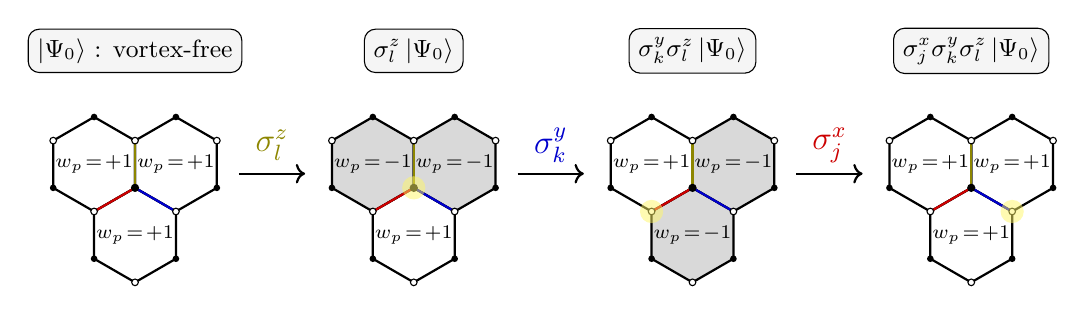
\begin{tikzpicture}[scale=0.6]
\newcommand{\hexcluster}[8]{
  \begin{scope}[shift={(#1,0)}]
    \node[draw,fill=black!4,rounded corners,font=\small] at (0,2.9) {#2};
    \fill[#3] (0,1)--(-0.866,1.5)--(-1.732,1)--(-1.732,0)--(-0.866,-0.5)--(0,0)--cycle; % Left
    \fill[#4] (0.866,1.5)--(0,1)--(0,0)--(0.866,-0.5)--(1.732,0)--(1.732,1)--cycle;      % Right
    \fill[#5] (0,0)--(-0.866,-0.5)--(-0.866,-1.5)--(0,-2)--(0.866,-1.5)--(0.866,-0.5)--cycle; % Bot
    \draw[thick] (0,1)--(-0.866,1.5)--(-1.732,1)--(-1.732,0)--(-0.866,-0.5)--(0,0)--cycle;
    \draw[thick] (0.866,1.5)--(0,1)--(0,0)--(0.866,-0.5)--(1.732,0)--(1.732,1)--cycle;
    \draw[thick] (0,0)--(-0.866,-0.5)--(-0.866,-1.5)--(0,-2)--(0.866,-1.5)--(0.866,-0.5)--cycle;
    \node[font=\scriptsize] at (-0.866,0.5) {$w_p\!=\!#6$};
    \node[font=\scriptsize] at ( 0.866,0.5) {$w_p\!=\!#7$};
    \node[font=\scriptsize] at (0,-1)        {$w_p\!=\!#8$};
    \draw[red!80!black, thick](0,0)--(-0.866,-0.5); % x = lower-left
    \draw[blue!80!black,thick](0,0)--(0.866,-0.5);  % y = lower-right
    \draw[olive,        thick](0,0)--(0,1);         % z = up
    \fill(0,0)circle(2.5pt); \fill(-0.866,1.5)circle(2pt); \fill(-1.732,0)circle(2pt);
    \fill(0.866,1.5)circle(2pt); \fill(1.732,0)circle(2pt);
    \fill(-0.866,-1.5)circle(2pt); \fill(0.866,-1.5)circle(2pt);
    \fill[white](0,1)circle(2pt);\draw(0,1)circle(2pt);
    \fill[white](-0.866,-0.5)circle(2pt);\draw(-0.866,-0.5)circle(2pt);
    \fill[white](0.866,-0.5)circle(2pt);\draw(0.866,-0.5)circle(2pt);
    \fill[white](-1.732,1)circle(2pt);\draw(-1.732,1)circle(2pt);
    \fill[white](1.732,1)circle(2pt);\draw(1.732,1)circle(2pt);
    \fill[white](0,-2)circle(2pt);\draw(0,-2)circle(2pt);
  \end{scope}
}

% ---------- PANEL 1 : initial, all +1 ----------
\hexcluster{0}{$|\Psi_0\rangle$ : vortex-free}
  {white}{white}{white}{+1}{+1}{+1}

\draw[->,thick] (2.2,0.3)--(3.6,0.3);
\node[olive,font=\large] at (2.9,0.9) {$\sigma^z_l$};

% ---------- PANEL 2 : after sigma^z -> flips Left + Right ----------
\hexcluster{5.9}{$\sigma^z_l\,|\Psi_0\rangle$}
  {gray!30}{gray!30}{white}{-1}{-1}{+1}
\fill[yellow!60,opacity=0.5] (5.9,0) circle(7pt);

\draw[->,thick] (8.1,0.3)--(9.5,0.3);
\node[blue!80!black,font=\large] at (8.8,0.9) {$\sigma^y_k$};

% ---------- PANEL 3 : after sigma^y at k -> flips Left + Bot ----------
\hexcluster{11.8}{$\sigma^y_k\sigma^z_l\,|\Psi_0\rangle$}
  {white}{gray!30}{gray!30}{+1}{-1}{-1}
\fill[yellow!60,opacity=0.5] (10.934,-0.5) circle(7pt);

\draw[->,thick] (14.0,0.3)--(15.4,0.3);
\node[red!80!black,font=\large] at (14.7,0.9) {$\sigma^x_j$};

% ---------- PANEL 4 : after sigma^x at j -> flips Right + Bot, all restored ----------
\hexcluster{17.7}{$\sigma^x_j\sigma^y_k\sigma^z_l\,|\Psi_0\rangle$}
  {white}{white}{white}{+1}{+1}{+1}
\fill[yellow!60,opacity=0.5] (18.566,-0.5) circle(7pt);

\end{tikzpicture}
\caption{The flux-restoring third-order process. Start from the vortex-free
  state $\ket{\Psi_0}$ (all $w_p=+1$, white). Each Zeeman operator
  $\sigma_i^\alpha$ at the highlighted site flips the two $w_p$ next to its
  $\alpha$-bond (grey, $w_p=-1$). Only the full product
  $\sigma_j^x\sigma_k^y\sigma_l^z$ returns all $w_p$ to $+1$; the
  intermediate one- and two-operator states lie outside the vortex-free
  sector and are projected out by $\Pi_0$. Bond colours: $x$ red, $y$ blue,
  $z$ olive.}
\label{fig:sm_flux_flip}
\end{figure}

%==============================================================================
\section{Reduction of the three-spin term to a Majorana bilinear}
\label{sm:nnn}

Insert the Majorana representation $\sigma^\alpha_j = \ii\,\hat
b^\alpha_j\oga_j$ into one triple of \cref{eq:sm_H3_spin}:
\begin{align}
  \sigma_j^x \sigma_k^y \sigma_l^z
  = (\ii\, \obx_j \oga_j)(\ii\, \oby_k \oga_k)(\ii\, \obz_l \oga_l)
  = -\ii\, \obx_j \oga_j\, \oby_k \oga_k\, \obz_l \oga_l .
\end{align}
On the central site $l$ we reduce the pair $\obz_l\oga_l$ by the
physical-subspace condition $\hat D_l=\obx_l\oby_l\obz_l\oga_l=1$. Moving
$\oga_l$ through the three $\hat b_l$'s gives $(-1)^3$, and $\oga_l^2=1$,
so
\begin{align}
  \obz_l \oga_l = \obz_l \oga_l\, \hat D_l
  = \obz_l\, \oga_l\, \obx_l \oby_l \obz_l \oga_l
  = -\,\obz_l\, \obx_l \oby_l \obz_l
  = -\,\obx_l \oby_l ,
\end{align}
where in the last step the first $\obz_l$ passes through $\obx_l\oby_l$ (two
anticommutations, sign $+1$) and $(\obz_l)^2=1$. Hence
\begin{align}
  \sigma_j^x \sigma_k^y \sigma_l^z
  = +\ii\, \obx_j \oga_j\, \oby_k \oga_k\, \obx_l \oby_l
  = +\ii\, (\obx_j \obx_l)(\oby_k \oby_l)(\oga_j \oga_k).
\end{align}
The reordering is an even permutation of six Majorana
operators, so the sign is $+1$. I track this sign carefully, since it fixes
the sign of the final hopping term. With the link operators $\hat u_{jl}=\ii\,\obx_j
\obx_l$ and $\hat u_{kl}=\ii\,\oby_k \oby_l$ (so $\obx_j\obx_l = -\ii\,\hat
u_{jl}$, $\oby_k\oby_l=-\ii\,\hat u_{kl}$),
\begin{align}
  \sigma_j^x \sigma_k^y \sigma_l^z
  = \ii\,(-\ii\,\hat u_{jl})(-\ii\,\hat u_{kl})\,\oga_j\oga_k
  = -\ii\, \hat u_{jl}\, \hat u_{kl}\, \oga_j \oga_k
  \;\xrightarrow{\ u_{jl}=u_{kl}=1\ }\;
  -\ii\, \oga_j \oga_k .
  \label{eq:sm_H3_triple}
\end{align}
The three-spin operator is now a next-nearest-neighbour Majorana
hopping between the two same-sublattice ($A$) sites $j,k$, displaced by
$\bm n_1-\bm n_2$ (\cref{fig:sm_nnn_hop}). The triples from the
other two bond pairs around a site give the displacements $\bm n_1$ and
$\bm n_2$. This imaginary second-neighbour hopping has the same
structure as the Haldane model \cite{Haldane1988}, here for Majorana
fermions.

\begin{figure}[H]
\centering
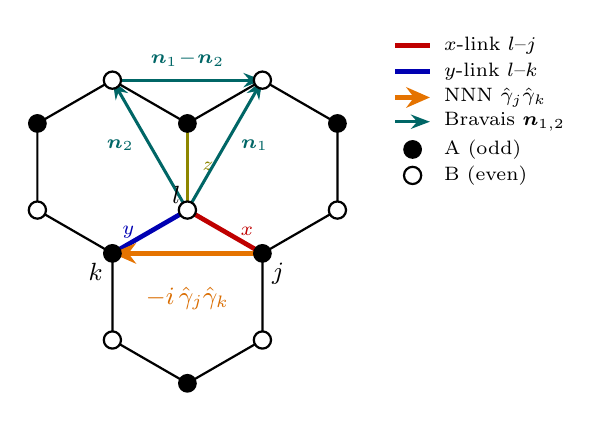
\begin{tikzpicture}[scale=1.1,
  Asite/.style={circle,fill,inner sep=2.4pt},
  Bsite/.style={circle,draw,fill=white,line width=0.8pt,inner sep=2.2pt},
  nnnhop/.style={line width=1.7pt,orange!90!black,
                 -{Stealth[length=3mm,width=2.6mm]}},
  nvec/.style={line width=1.1pt,teal!80!black,-{Stealth[length=2.4mm]}}]

  % ===== three hexagons sharing centre l at (0,0) =====
  \draw[thick] (0,1)--(-0.866,1.5)--(-1.732,1)--(-1.732,0)--(-0.866,-0.5)--(0,0)--cycle;
  \draw[thick] (0.866,1.5)--(0,1)--(0,0)--(0.866,-0.5)--(1.732,0)--(1.732,1)--cycle;
  \draw[thick] (0,0)--(-0.866,-0.5)--(-0.866,-1.5)--(0,-2)--(0.866,-1.5)--(0.866,-0.5)--cycle;

  % ===== NN links of the triple: l-j (x), l-k (y) =====
  \draw[line width=1.7pt,red!75!black]  (0,0)--(0.866,-0.5)
     node[midway,right=1.5pt,font=\scriptsize]{$x$};
  \draw[line width=1.7pt,blue!70!black] (0,0)--(-0.866,-0.5)
     node[midway,left=1.5pt,font=\scriptsize]{$y$};
  \draw[line width=1.2pt,olive] (0,0)--(0,1)
     node[midway,right=1.5pt,font=\scriptsize]{$z$};

  % ===== NNN effective hopping j <-> k =====
  \draw[nnnhop] (0.866,-0.5) to(-0.866,-0.5);
  \node[orange!85!black,font=\small] at (0,-1.02) {$-i\,\oga_j \oga_k$};

  % ===== n1, n2 direction vectors from centre l =====
  \draw[nvec] (0,0)--(0.866,1.5)  node[midway,right=2pt,font=\scriptsize,teal!80!black]{$\bm n_1$};
  \draw[nvec] (0,0)--(-0.866,1.5) node[midway,left=2pt,font=\scriptsize,teal!80!black]{$\bm n_2$};
  \draw[nvec] (-0.866,1.5)--(0.866,1.5)
     node[midway,above=1pt,font=\scriptsize,teal!80!black]{$\bm n_1\!-\!\bm n_2$};
  % ===== sites =====
  \node[Bsite] at (0,0){};
  \node[Bsite] at (-0.866,1.5){}; \node[Bsite] at (-1.732,0){};
  \node[Bsite] at (0.866,1.5){};  \node[Bsite] at (1.732,0){};
  \node[Bsite] at (-0.866,-1.5){};\node[Bsite] at (0.866,-1.5){};
  \node[Asite] at (0,1){};
  \node[Asite] at (0.866,-0.5){};
  \node[Asite] at (-0.866,-0.5){};
  \node[Asite] at (-1.732,1){}; \node[Asite] at (1.732,1){}; \node[Asite] at (0,-2){};

  % ===== labels =====
  \node[font=\small,above left=-1pt] at (0,0) {$l$};
  \node[font=\small,below right=0pt] at (0.866,-0.5) {$j$};
  \node[font=\small,below left=0pt]  at (-0.866,-0.5) {$k$};

  % ===== legend =====
  \begin{scope}[shift={(2.4,1.1)}]
    \draw[line width=1.7pt,red!75!black]  (0,0.8)--(0.4,0.8);
    \node[right,font=\scriptsize] at (0.45,0.8){$x$-link $l$–$j$};
    \draw[line width=1.7pt,blue!70!black] (0,0.5)--(0.4,0.5);
    \node[right,font=\scriptsize] at (0.45,0.5){$y$-link $l$–$k$};
    \draw[nnnhop] (0,0.2)--(0.4,0.2);
    \node[right,font=\scriptsize] at (0.45,0.2){NNN $\oga_j\oga_k$};
    \draw[nvec] (0,-0.08)--(0.4,-0.08);
    \node[right,font=\scriptsize] at (0.45,-0.08){Bravais $\bm n_{1,2}$};
    \node[Asite] at (0.2,-0.4){}; \node[right,font=\scriptsize] at (0.45,-0.4){A (odd)};
    \node[Bsite] at (0.2,-0.7){}; \node[right,font=\scriptsize] at (0.45,-0.7){B (even)};
  \end{scope}

\end{tikzpicture}
\caption{Next-nearest-neighbour Majorana hopping from the third-order
  perturbation. The three-spin operator $\sigma_j^x\sigma_k^y\sigma_l^z$
  acts on a triple sharing the central even ($B$) site $l$, joined by its
  $x$- and $y$-links to the two odd ($A$) sites $j,k$. In the fixed gauge
  $u_{jk}=1$ it becomes a next-nearest-neighbour hopping
  $-\ii\,\oga_j\oga_k$ (orange) between the two same-sublattice sites
  $j,k$, displaced by $\bm n_1-\bm n_2$.}
\label{fig:sm_nnn_hop}
\end{figure}

%==============================================================================
\section{The mass term \texorpdfstring{$d_z(\bm q)$}{dz(q)} and the gap}
\label{sm:dz}

Write $\oga_j\to\oga^A_{\bm R}$ and $\oga_k\to\oga^A_{\bm R+\bm n}$ with
$\bm n\in\{\bm n_1,\bm n_2,\bm n_1-\bm n_2\}$. An $A$-centred process
carries the opposite sign on the $B$ sublattice, since the directed bond
reverses: $\hat u_{l'j'}=-\hat u_{j'l'}$. The third-order contribution then takes the same
$\tfrac{\ii}{4}\sum A_{jk}\oga_j\oga_k$ form as the nearest-neighbour
Hamiltonian:
\begin{align}
  H^{(3)}_{\text{eff}} = \frac{\ii}{4}\,\kappa \sum_{\bm R}\sum_{\bm n}
  \left[\oga_{\bm R}^{A}\,\oga_{\bm R+\bm n}^{A}
      - \oga_{\bm R}^{B}\,\oga_{\bm R+\bm n}^{B}\right],
  \qquad
  \bm n \in \{\bm n_1,\ \bm n_2,\ \bm n_1-\bm n_2\} .
  \label{eq:sm_H3_realspace}
\end{align}

Both operators of a same-sublattice term share the offset $\bm\delta_z$ (or
none). The shared offset cancels under momentum conservation, so we
transform with the cell label only, $\oga^{A}_{\bm R}=\tfrac{1}{\sqrt N}\sum_{\bm
q}\ee^{\ii\bm q\cdot\bm R}\tilde\gamma^A_{\bm q}$. Substituting,
\begin{align}
  H^{AA}
  &= \kappa\frac{\ii}{4}\sum_{\bm n}\sum_{\bm R}\oga_{\bm R}^{A}\,\oga_{\bm R+\bm n}^{A}
  = \kappa\frac{\ii}{4}\sum_{\bm n}\frac{1}{N}\sum_{\bm q,\bm q'}\ee^{\ii\bm q'\cdot\bm n}\,\tilde\gamma_{\bm q}^{A}\tilde\gamma_{\bm q'}^{A}\underbrace{\sum_{\bm R}\ee^{\ii(\bm q+\bm q')\cdot\bm R}}_{N\,\delta_{\bm q+\bm q',\,0}} \notag\\
  &= \kappa\frac{\ii}{4}\sum_{\bm n}\sum_{\bm q}\ee^{-\ii\bm q\cdot\bm n}\,\tilde\gamma_{\bm q}^{A}\tilde\gamma_{-\bm q}^{A}.
\end{align}

The two operators now live on the same sublattice, so
$\tilde\gamma_{-\bm q}^{A}\tilde\gamma_{\bm q}^{A} = -\tilde\gamma_{\bm
q}^{A}\tilde\gamma_{-\bm q}^{A}$. The bilinear is odd under $\bm
q\to-\bm q$. We symmetrize the $\bm q$-sum by relabelling $\bm q\to-\bm q$
in one half:
\begin{align}
  \sum_{\bm q}\ee^{-\ii\bm q\cdot\bm n}\,\tilde\gamma_{\bm q}^{A}\tilde\gamma_{-\bm q}^{A}
  &= \tfrac12\sum_{\bm q}\Big(\ee^{-\ii\bm q\cdot\bm n}\,\tilde\gamma_{\bm q}^{A}\tilde\gamma_{-\bm q}^{A}+\ee^{+\ii\bm q\cdot\bm n}\,\tilde\gamma_{-\bm q}^{A}\tilde\gamma_{\bm q}^{A}\Big) \notag\\
  &= \tfrac12\sum_{\bm q}\big(\ee^{-\ii\bm q\cdot\bm n}-\ee^{+\ii\bm q\cdot\bm n}\big)\tilde\gamma_{\bm q}^{A}\tilde\gamma_{-\bm q}^{A}
   = -\ii\sum_{\bm q}\sin(\bm q\cdot\bm n)\,\tilde\gamma_{\bm q}^{A}\tilde\gamma_{-\bm q}^{A}.
\end{align}
In the nearest-neighbour $A$--$B$ block the sublattices are distinct, so
the full exponential $f(\bm q)$ survives. The relevant dot
products are
\begin{align}
  \bm q\cdot\bm n_1=\tfrac{\sqrt3}{2}q_x+\tfrac32 q_y,\qquad
  \bm q\cdot\bm n_2=-\tfrac{\sqrt3}{2}q_x+\tfrac32 q_y,\qquad
  \bm q\cdot(\bm n_1-\bm n_2)=\sqrt3\,q_x .
\end{align}
Thus $H^{AA}=\tfrac{\kappa}{4}\sum_{\bm q}\big[\sum_{\bm n}\sin(\bm
q\cdot\bm n)\big]\tilde\gamma^A_{\bm q}\tilde\gamma^A_{-\bm q}$. Plugging
into the Bloch form $\tfrac12\sum_{\bm q}\chi^\dag_{\bm q}h(\bm
q)\chi_{\bm q}$, the upper-left ($A$--$A$) diagonal entry gives
$d_z(\bm q)$ up to a positive $O(1)$ factor. The coupling $\kappa\sim
h^xh^yh^z/\abs{J}^2$ is only fixed up to such a factor. We absorb this
factor and the overall sign into $\kappa$. The mass term is
\begin{align}
  d_z(\bm q) = 6\kappa\Big[\sin(\bm q\cdot\bm n_1) + \sin(\bm q\cdot\bm n_2)
  + \sin\!\big(\bm q\cdot(\bm n_1-\bm n_2)\big)\Big].
  \label{eq:sm_dz}
\end{align}
The $B$-sublattice block carries the opposite sign in
\cref{eq:sm_H3_realspace} and gives the lower-right entry $-d_z(\bm q)$.
Together the two blocks give $d_z(\bm q)\,\sigma_z$, and the Bloch
Hamiltonian becomes
\begin{align}
  h(\bm q)=\begin{pmatrix} d_z(\bm q) & \ii f(\bm q)\\[2pt] -\ii f^*(\bm q) & -d_z(\bm q)\end{pmatrix}
  =\bm d(\bm q)\cdot\bm\sigma,
  \qquad
  \varepsilon_\pm(\bm q)=\pm\sqrt{\abs{f(\bm q)}^2+d_z(\bm q)^2},
  \label{eq:sm_h_gapped}
\end{align}
since $d_x^2+d_y^2=\abs{f}^2$ is unchanged.

As a sum of sines, $d_z$ is odd, $d_z(-\bm q)=-d_z(\bm q)$,
consistent with broken time reversal by \cref{eq:sm_d_parity}. At $\bm
K=(-\tfrac{2\pi}{3\sqrt3},\tfrac{2\pi}{3})$ the three phases are
\begin{align}
  \bm K\cdot\bm n_1=\tfrac{2\pi}{3},\qquad
  \bm K\cdot\bm n_2=\tfrac{4\pi}{3},\qquad
  \bm K\cdot(\bm n_1-\bm n_2)=-\tfrac{2\pi}{3},
\end{align}
so
\begin{align}
  d_z(\bm K) &= 6\kappa\Big[\sin\tfrac{2\pi}{3}+\sin\tfrac{4\pi}{3}+\sin\big(\!-\tfrac{2\pi}{3}\big)\Big]
  = 6\kappa\Big(\tfrac{\sqrt3}{2}-\tfrac{\sqrt3}{2}-\tfrac{\sqrt3}{2}\Big)
  = -3\sqrt3\,\kappa, \notag\\
  \Delta &= 2\abs{d_z(\bm K)} = 6\sqrt3\,\abs{\kappa}.
  \label{eq:sm_gap_value}
\end{align}
By oddness $d_z(-\bm K)=+3\sqrt3\,\kappa$, so the two Dirac points have
opposite masses,
\begin{align}
  m_{\pm\bm K} \equiv d_z(\pm\bm K) = \mp 3\sqrt3\,\kappa .
  \label{eq:sm_masses}
\end{align}
This is the same mechanism as the Haldane model \cite{Haldane1988}. The gap opening is shown
in \cref{fig:sm_gap_opening}.

\begin{figure}[H]
  \centering
  \includegraphics[width=0.95\textwidth]{HC_3_gap_opening.pdf}
  \caption{Topological gap opening at the Dirac point $\bm K$. \emph{Left}: the field-induced mass
  $d_z(\bm q)$ gaps the dispersion $\varepsilon_\pm=\pm\sqrt{\abs{f}^2+d_z^2}$.
  \emph{Right}: a one-dimensional cut through
  $\bm K$ for increasing $\kappa$, with $\varepsilon_+$ (solid) and
  $\varepsilon_-$ (dashed) splitting apart as the gap opens.}
  \label{fig:sm_gap_opening}
\end{figure}

%==============================================================================
\section{Calculation of Chern number}
\label{sm:chern}

The invariant of the gapped phase is the Chern number of the occupied band
\cite{TKNN1982},
\begin{align}
  \C=\frac{1}{2\pi}\int_{\text{BZ}}\Omega(\bm q)\,\dd^2q,\qquad
  \Omega=\pp_{q_x}A_y-\pp_{q_y}A_x,\qquad
  A_\mu(\bm q)=-\ii\,\langle u_-\vert\pp_{q_\mu}u_-\rangle,
  \label{eq:sm_chern_def}
\end{align}
with $\ket{u_-}$ the normalized negative-energy eigenstate of $h(\bm
q)$.

Parametrize the unit vector as
\begin{align}
  \hat{\bm d}=(\sin\theta\cos\phi,\ \sin\theta\sin\phi,\ \cos\theta),
  \qquad
  \cos\theta=\frac{d_z}{\abs{\bm d}},
  \qquad
  \ee^{\ii\phi}=\frac{d_x+\ii d_y}{\sqrt{d_x^2+d_y^2}},
\end{align}
where $d_x+\ii d_y=-\ii f^*(\bm q)$ by \cref{eq:sm_dvector}. The
lower-band eigenstate in one gauge is
\begin{align}
  \ket{u_-}=\begin{pmatrix}\sin\tfrac\theta2\,\ee^{-\ii\phi}\\[3pt]-\cos\tfrac\theta2\end{pmatrix},
\end{align}
which satisfies $(\hat{\bm d}\cdot\bm\sigma)\ket{u_-}=-\ket{u_-}$. One
can check this by direct multiplication using $\hat{\bm d}\cdot\bm\sigma=
\big[\begin{smallmatrix}\cos\theta & \sin\theta\,\ee^{-\ii\phi}\\
\sin\theta\,\ee^{\ii\phi} & -\cos\theta\end{smallmatrix}\big]$. Here I choose this gauge because it is smooth at the north pole
$\theta=0$; it is singular at $\theta=\pi$, but a second patch covers that
point, and $\C$ does not depend on the patch.
With $s=\sin\tfrac\theta2$, $c=\cos\tfrac\theta2$,
\begin{align}
  \pp_\mu\ket{u_-}=\begin{pmatrix}\ee^{-\ii\phi}\big(\tfrac12 c\,\pp_\mu\theta-\ii s\,\pp_\mu\phi\big)\\[3pt]\tfrac12 s\,\pp_\mu\theta\end{pmatrix},
  \qquad
  \bra{u_-}=\big(s\,\ee^{+\ii\phi},\;-c\big).
\end{align}
Term by term,
\begin{align}
  \langle u_-\vert\pp_\mu u_-\rangle
  &= s\,\ee^{\ii\phi}\ee^{-\ii\phi}\big(\tfrac12 c\,\pp_\mu\theta-\ii s\,\pp_\mu\phi\big)
   -c\big(\tfrac12 s\,\pp_\mu\theta\big) \notag\\
  &= \tfrac12 sc\,\pp_\mu\theta-\ii s^2\,\pp_\mu\phi-\tfrac12 sc\,\pp_\mu\theta
  = -\ii\,s^2\,\pp_\mu\phi .
\end{align}
The $\tfrac12 sc\,\pp_\mu\theta$ terms cancel, so
\begin{align}
  A_\mu=-\ii\,\langle u_-\vert\pp_\mu u_-\rangle = -\,s^2\,\pp_\mu\phi
  = -\tfrac12(1-\cos\theta)\,\pp_\mu\phi .
  \label{eq:sm_berry_connection}
\end{align}
Take the curl with $g\equiv\tfrac12(1-\cos\theta)$ and
$\pp_\mu g=\tfrac12\sin\theta\,\pp_\mu\theta$. The mixed second derivatives
of $\phi$ cancel, so
\begin{align}
  \Omega=-\big[(\pp_x g)(\pp_y\phi)-(\pp_y g)(\pp_x\phi)\big]
  =-\tfrac12\sin\theta\big(\pp_x\theta\,\pp_y\phi-\pp_y\theta\,\pp_x\phi\big)
  = -\tfrac12\,\hat{\bm d}\cdot\big(\pp_{q_x}\hat{\bm d}\times\pp_{q_y}\hat{\bm d}\big).
  \label{eq:sm_berry_curvature}
\end{align}
The last equality is the solid-angle Jacobian identity $\hat{\bm
d}\cdot(\pp_x\hat{\bm d}\times\pp_y\hat{\bm
d})=\sin\theta(\pp_x\theta\,\pp_y\phi-\pp_y\theta\,\pp_x\phi)$. The Chern
number is (minus) the degree of the map $\bm q\mapsto\hat{\bm d}$,
\begin{align}
  \C=-\frac{1}{4\pi}\int_{\text{BZ}}\hat{\bm d}\cdot\big(\pp_{q_x}\hat{\bm d}\times\pp_{q_y}\hat{\bm d}\big)\,\dd^2q .
  \label{eq:sm_chern_winding}
\end{align}

For the gapped cones we also need the in-plane winding
\begin{align}
  \nu_i=\frac{1}{2\pi}\oint_{\mathcal C_i}\dd\big(\arg f(\bm q)\big)
\end{align}
around each Dirac point. From the linearization \cref{eq:sm_linearization},
$f(\bm K+\delta\bm q)\propto(\delta q_x-\ii\,\delta q_y)$. Its phase
winds by $-2\pi$ on a counterclockwise loop, so $\nu_{\bm K}=-1$. At $-\bm K$,
$f(-\bm K+\delta\bm q)=f(\bm K-\delta\bm q)^*\propto(\delta q_x+\ii\,\delta
q_y)$, so $\nu_{-\bm K}=+1$. The two windings are opposite:
the total winding over the Brillouin-zone torus must vanish
(Nielsen--Ninomiya \cite{NielsenNinomiya1981}), so Dirac points come in
pairs of opposite chirality.

Near $\bm K_i$ write $f\simeq v\,\ee^{\ii\beta_i}(\delta q_x+\ii\,\nu_i\,
\delta q_y)$ with $v=\tfrac{3J}{2}$. The constant phase $\beta_i$ only
rotates $(d_x,d_y)$ in the plane and drops out of the triple product, so
we set $\beta_i=0$. With $m_i=d_z(\bm K_i)$ constant to leading order,
\begin{align}
  \bm d(\bm K_i+\delta\bm q)
  = \big(-\operatorname{Im}f,\ -\operatorname{Re}f,\ m_i\big)
  = \big(-v\,\nu_i\,\delta q_y,\ -v\,\delta q_x,\ m_i\big) .
\end{align}
The triple product is constant:
\begin{align}
  \pp_x\bm d &= (0,-v,0),\qquad \pp_y\bm d=(-v\nu_i,0,0)
  \;\Longrightarrow\;
  \pp_x\bm d\times\pp_y\bm d=(0,0,-v^2\nu_i), \notag\\
  \bm d\cdot(\pp_x\bm d\times\pp_y\bm d) &= -v^2\nu_i\,m_i .
\end{align}
Normalizing by $\abs{\bm d}^3=(v^2\rho^2+m_i^2)^{3/2}$ and integrating in
polar coordinates $\delta\bm q=\rho(\cos\alpha,\sin\alpha)$,
\begin{align}
  \C_i &= -\frac{1}{4\pi}\int \frac{-v^2\nu_i m_i}{(v^2\rho^2+m_i^2)^{3/2}}\,\dd^2\delta q
  =\frac{\nu_i m_i}{4\pi}\,(2\pi)\int_0^\infty\frac{v^2\rho\,\dd\rho}{(v^2\rho^2+m_i^2)^{3/2}} \notag\\
  &= \frac{\nu_i m_i}{2}\Big[\frac{-1}{\sqrt{v^2\rho^2+m_i^2}}\Big]_0^\infty
  =\tfrac12\,\nu_i\,\sgn(m_i).
\end{align}
Each cone contributes half a unit of Chern number. Summing,
\begin{align}
  \C=\tfrac12\sum_{i=\pm\bm K}\sgn(m_i)\,\nu_i .
  \label{eq:sm_chern_dirac}
\end{align}

From \cref{eq:sm_masses}, $\sgn(m_{\pm\bm K})=\mp\sgn(\kappa)$, and
$\nu_{\pm\bm K}=\mp1$ from above:
\begin{align}
  \C=\tfrac12\Big[\big(-\sgn\kappa\big)(-1)+\big(+\sgn\kappa\big)(+1)\Big]
  =\sgn(\kappa)=\sgn(h^xh^yh^z) ,
  \qquad
  \boxed{\;\C=\pm1=\sgn(\kappa) . \;}
  \label{eq:sm_chern_value}
\end{align}
If $d_z$ is even (the time-reversal-symmetric case of
\cref{eq:sm_d_parity}), the two masses are equal, $m_{-\bm K}=m_{\bm K}$.
The windings still obey $\nu_{\bm K}=-\nu_{-\bm K}$. Then
\begin{align}
  \C=\tfrac12\,\sgn(m_{\bm K})\big(\nu_{\bm K}+\nu_{-\bm K}\big)=0 .
\end{align}
The two half-integer contributions cancel and the gap is trivial. This
confirms \cref{sm:trs}: a nonzero Chern number requires the time-reversal breaking mass.

%==============================================================================
\bibliographystyle{apsrev4-2}
\bibliography{references}

\end{document}
